\documentclass{beamer}
\usepackage{pdfpages}
\usepackage{amssymb}
\usepackage{enumerate}
\usepackage{array}
\usepackage{lmodern}
\usepackage[all]{xy}
\definecolor{türkis}{rgb}{0.0, 0.65, 0.76}
\definecolor{weiss}{rgb}{1.0,1.0,1.0}
\usetheme{metropolis}
%\usecolortheme{whale}
\setbeamercolor{progress bar}{fg=türkis,bg=türkis}
\setbeamercolor{frametitle}{bg = türkis}
\setbeamercolor{background canvas}{bg = weiss}
\setbeamercolor{footline}{fg=gray}
\setbeamerfont{page number in head/foot}{size=\tiny}
\setbeamercolor{title}{fg = black}
\setbeamertemplate{frame footer}{ \insertlogo{
\includegraphics[width=1cm]{img/logo}} \hfill  \insertsection }
% \setbeamertemplate{navigation symbols}{\insertframenavigationsymbol}

\title[Denial-of-Service Angriffe]{Denial-of-Service Angriffe}
\subtitle{Ablauf, Wirkungsweise \& Auswahl konkreter Angriffe}
\institute{TU Ilmenau}
\date{06.05.2021}

\AtBeginSection[]
{
	\begin{frame}
		\frametitle{Gliederung}
		\tableofcontents[currentsection]
	\end{frame}
}

\begin{document}

\frame{\titlepage}

\section{Begriffserklärung \& Grundwissen}
\begin{frame}
	\frametitle{Was ist eine (D)DoS Attacke?}
	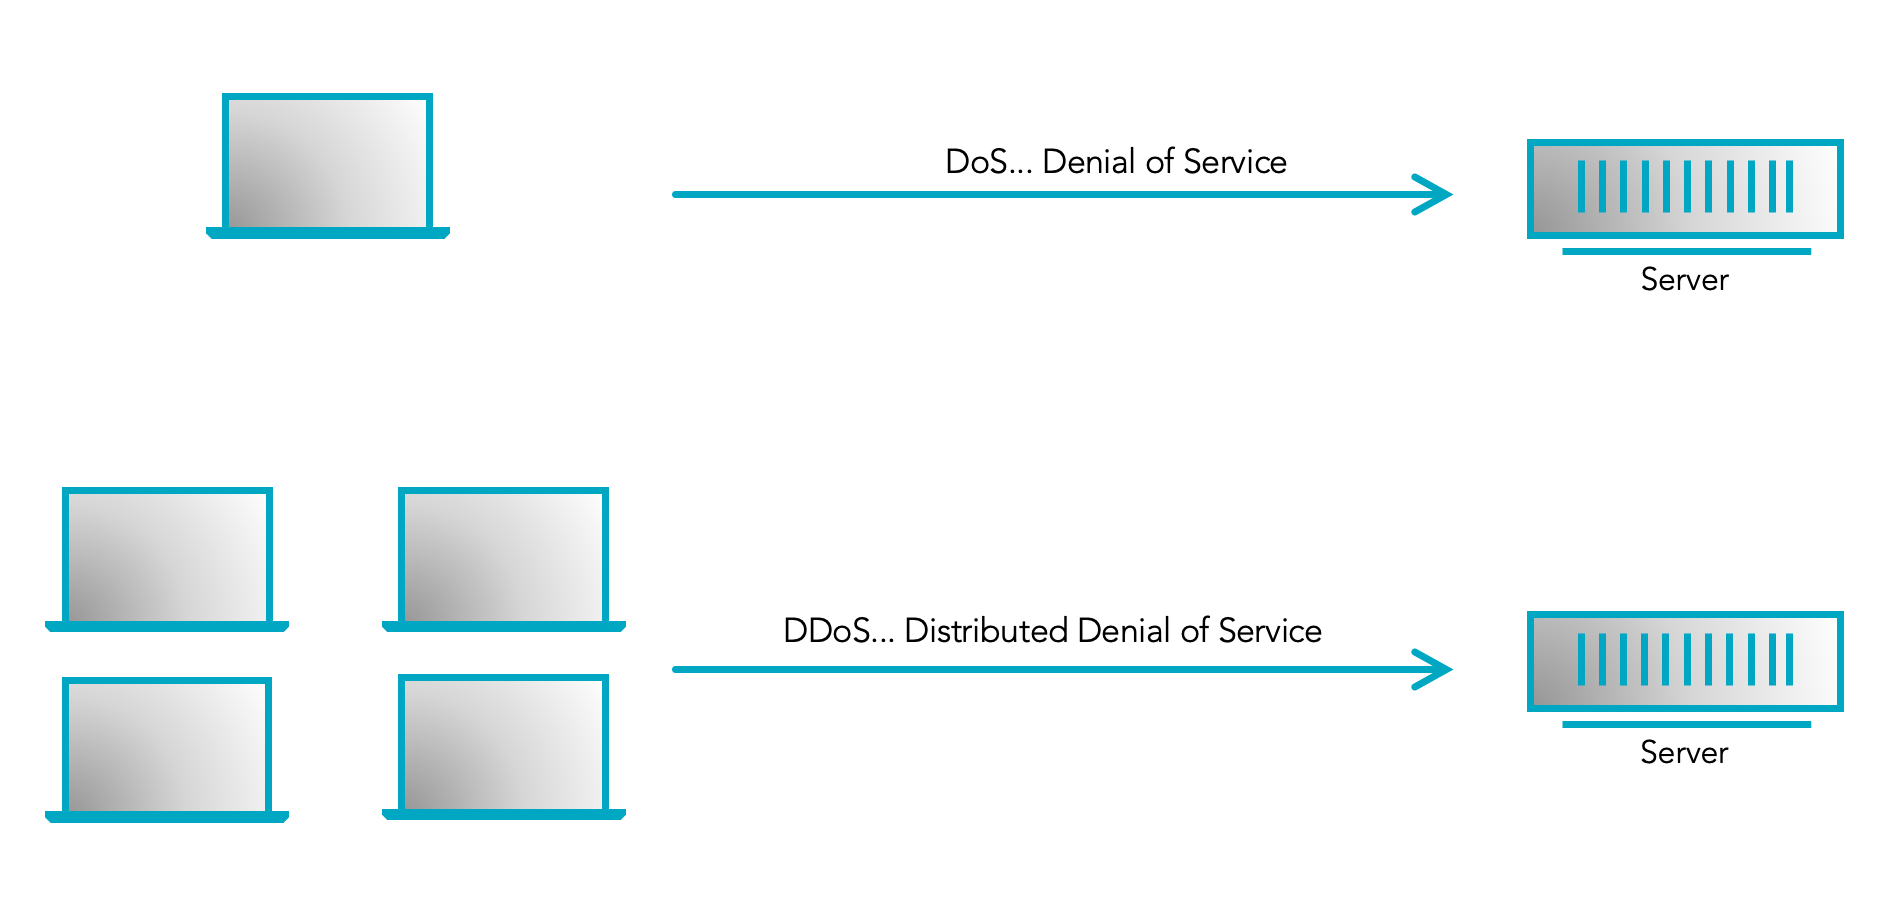
\includegraphics[width=0.9\linewidth]{img/1}
\end{frame}

\begin{frame}
	\frametitle{TCP 3-Wege-Handshake: Verbindungsaufbau}
	\begin{center}
		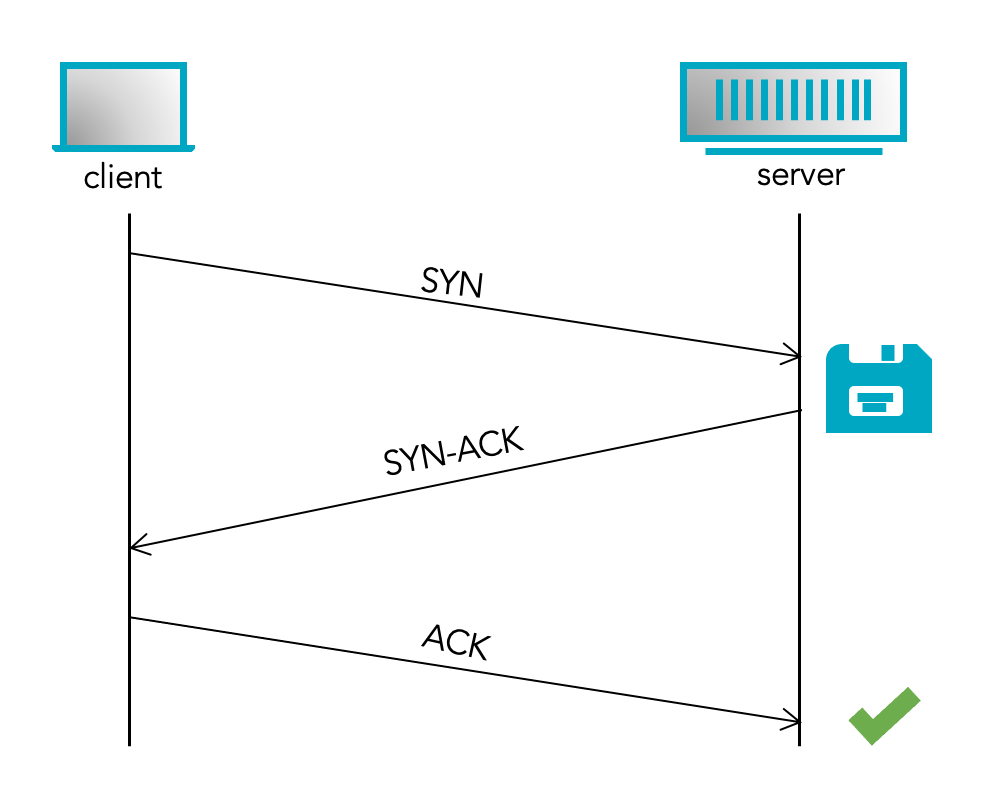
\includegraphics[width=0.9\linewidth]{img/2}
	\end{center}
\end{frame}

\begin{frame}
	\frametitle{TCP 3-Wege-Handshake: Verbindungsabbau}
	\begin{center}
		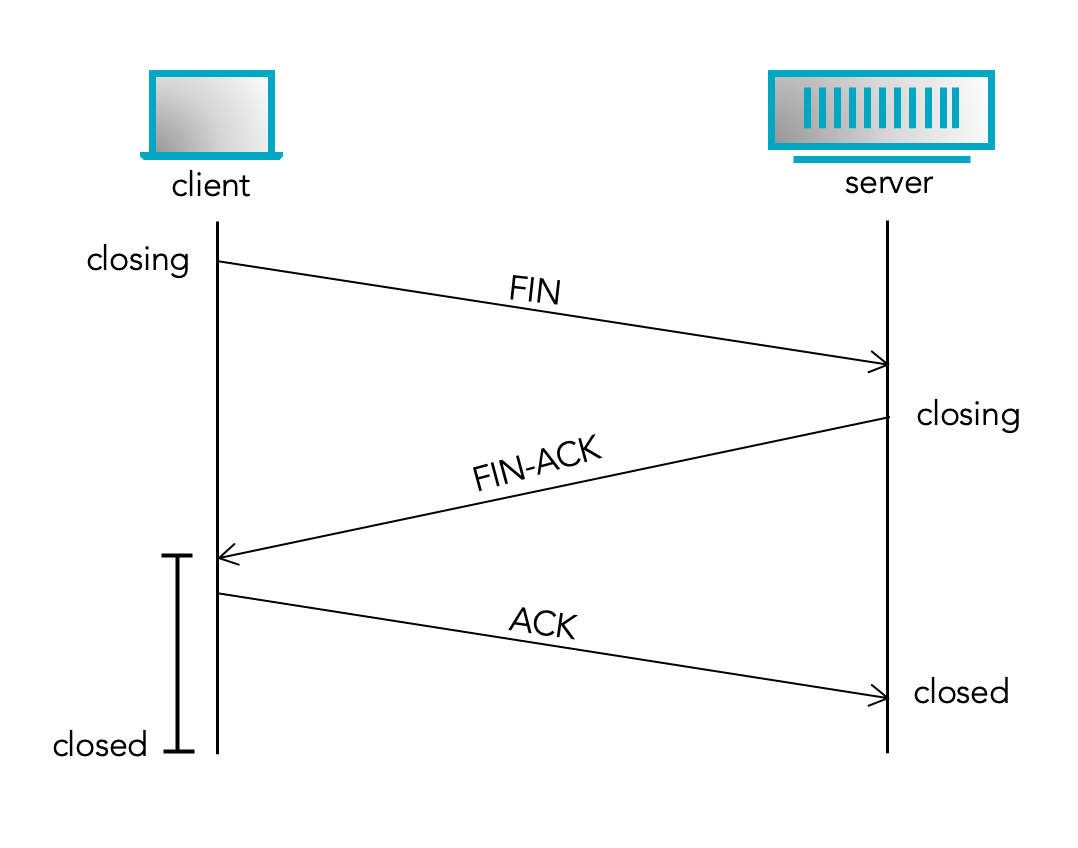
\includegraphics[width=0.9\linewidth]{img/3}
	\end{center}
\end{frame}

\section{Angriffsarten \& Abwehrmechanismen}
\begin{frame}
	\frametitle{SYN-Flooding}
	\begin{center}
		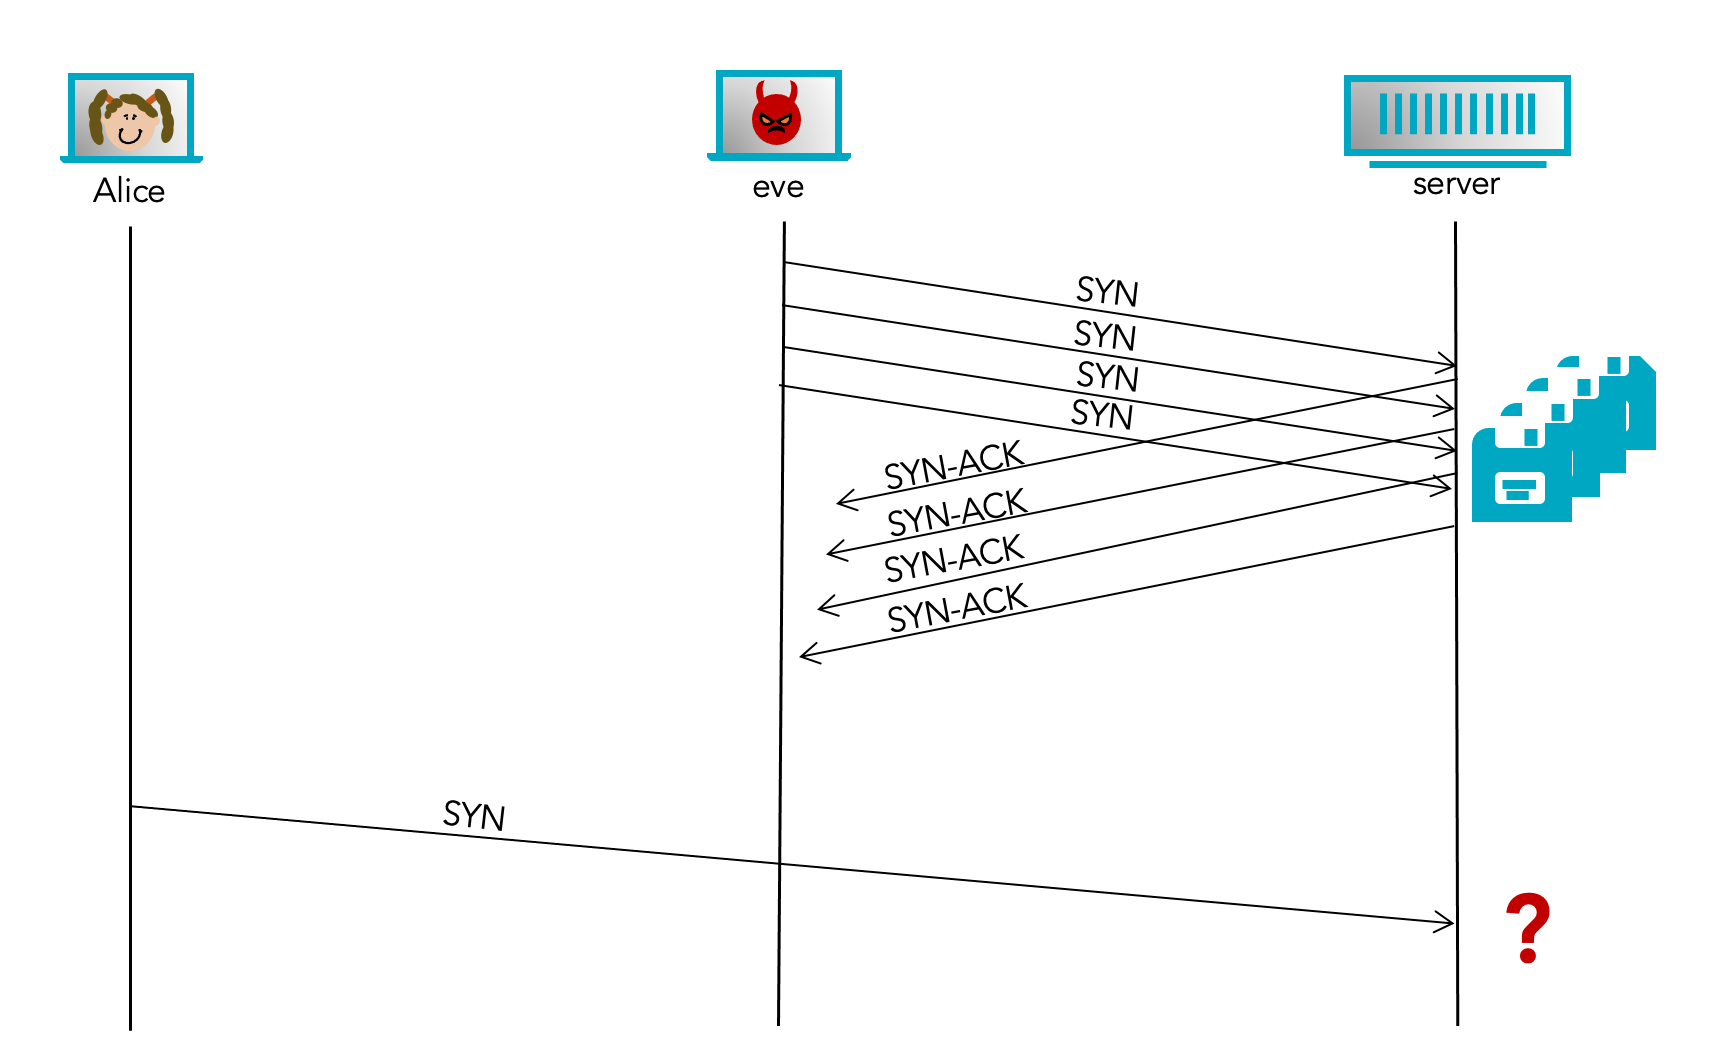
\includegraphics[width=0.9\linewidth]{img/4}
	\end{center}
\end{frame}

\begin{frame}
	\frametitle{Abwehrmechanismen: SYN-Flooding}
	\begin{itemize}
		\item Vergrößern des SYN-Backlogs
		\item Recycling der ältesten halboffenen TCP-Verbindung
		\item SYN-Cookies % (erweitert TCP um Regeln zur Sequenznummernvergabe und ermöglicht so die Auslagerung der Informationen über die halboffenen Verbindungen direkt in die Pakete)
		\item SYN-Caches %(Allokation minimaler Ressourcen für halboffene Verbindungen. allokation aller Ressourcen erst bei erfolgreichem Aufbau)
		\item Ingress Filter (Antispoofing) (Kann nur der ISP)
	\end{itemize}
\end{frame}

\begin{frame}
	\frametitle{SYN-FIN-Attack}
	\begin{center}
		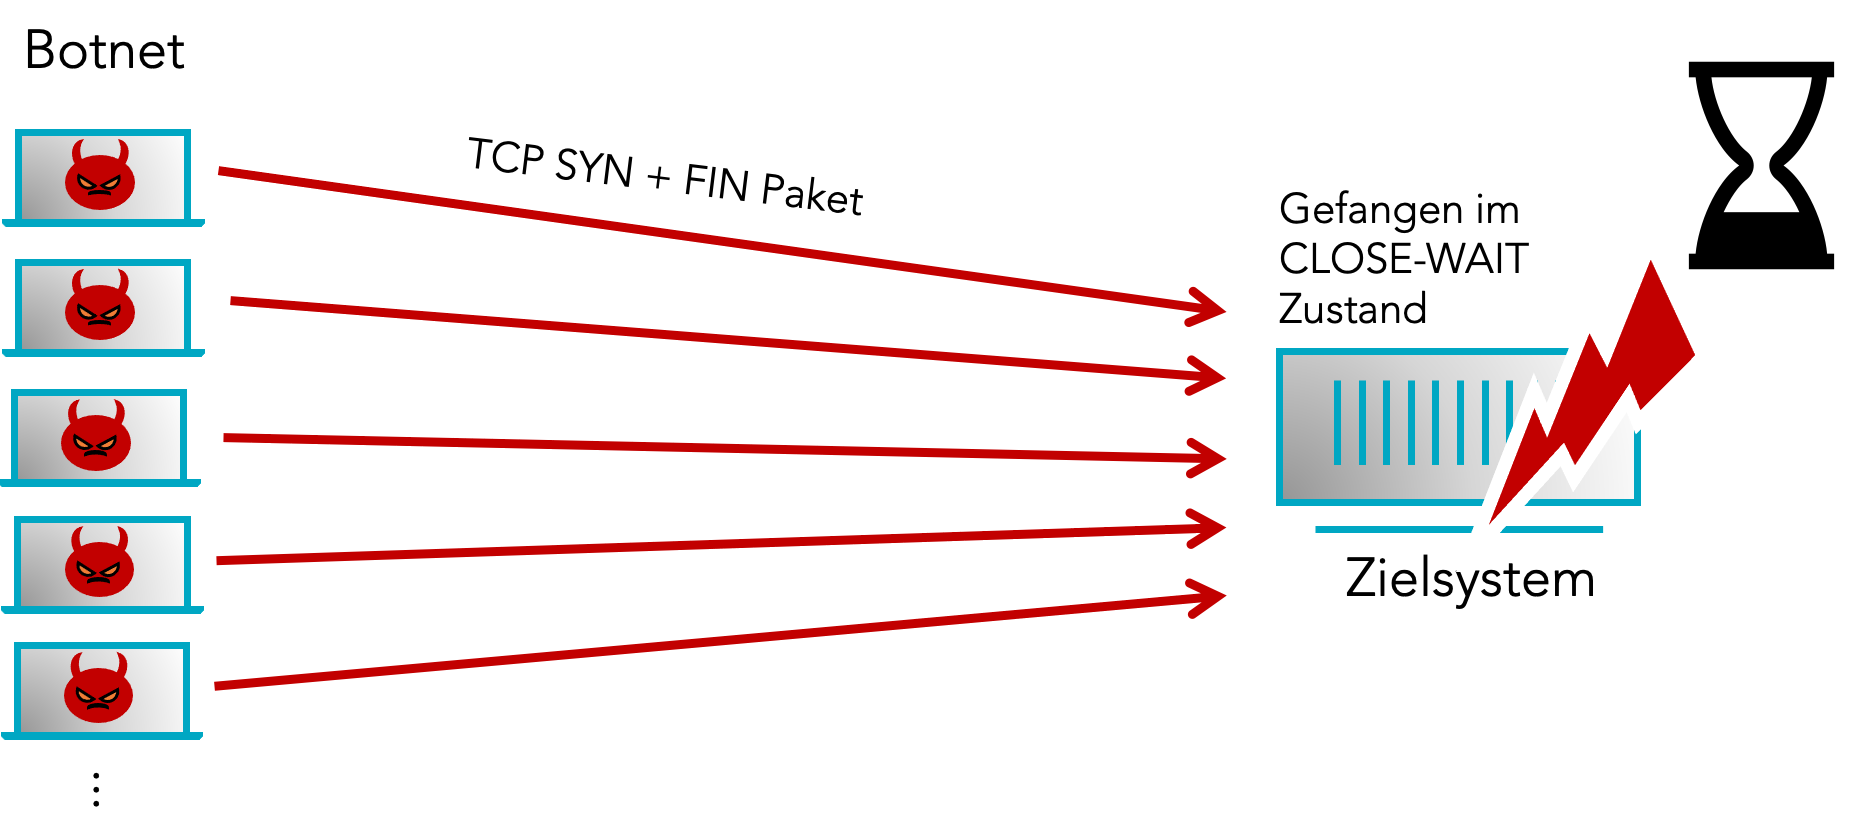
\includegraphics[width=0.9\linewidth]{img/9}
	\end{center}
\end{frame}

\begin{frame}
	\frametitle{Abwehrmechanismen: SYN-FIN-Attack}
	\begin{itemize}
		\item Verwerfen aller Pakete, welche sowohl SYN als auch FIN gesetzt haben.
	\end{itemize}
\end{frame}

\begin{frame}
	\frametitle{SYN-Frag-Attack }
	\begin{center}
		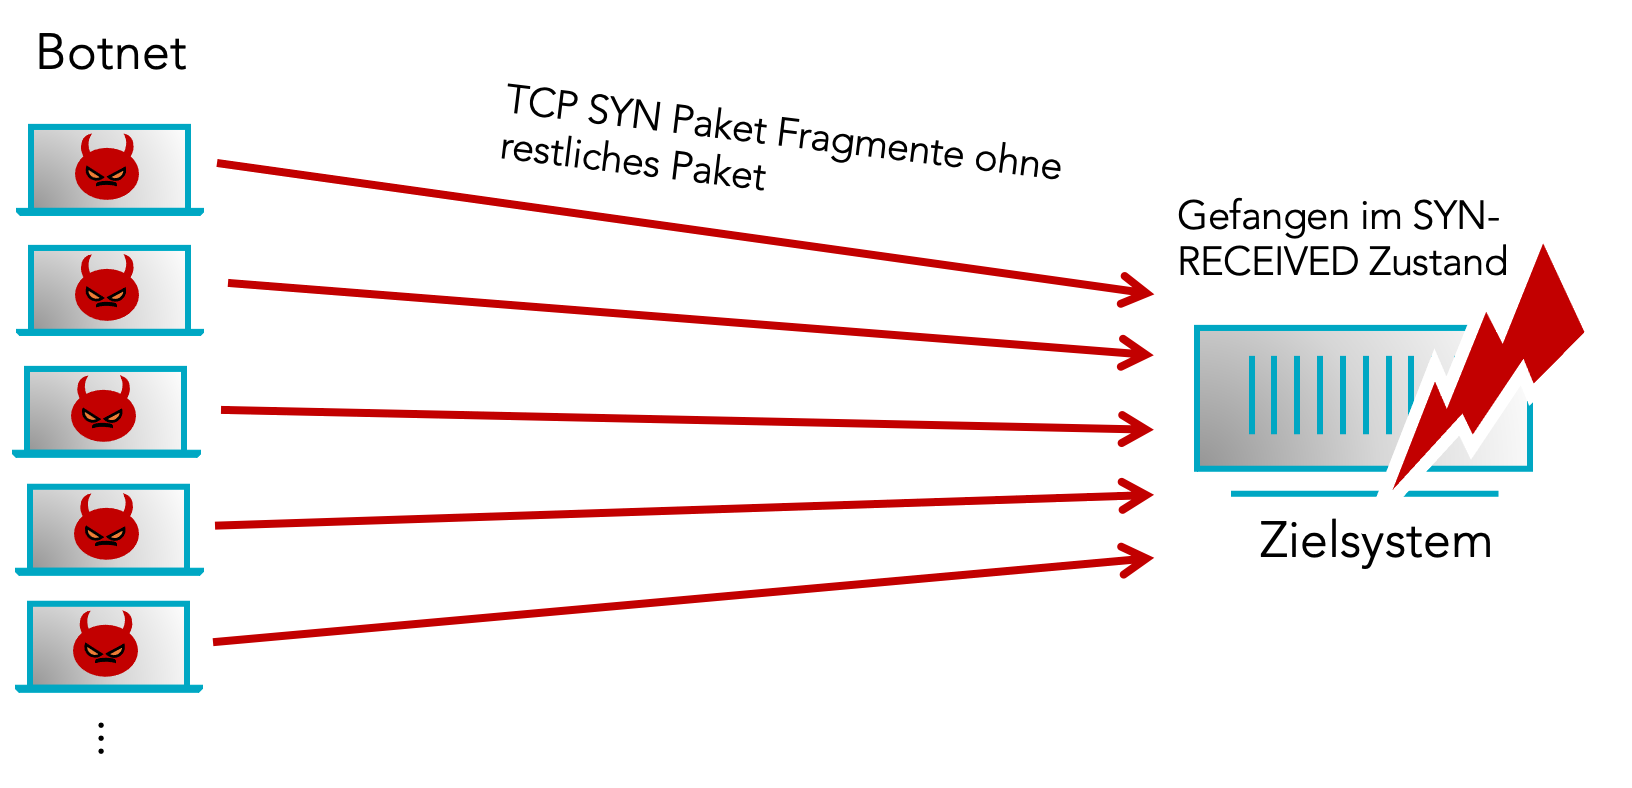
\includegraphics[width=0.9\linewidth]{img/syn}
	\end{center}
\end{frame}

\begin{frame}
	\frametitle{Abwehrmechanismen: SYN-Frag-Attack }
	\begin{itemize}
		\item Verwerfen segmentierter TCP SYN Pakete. % A 'SYN fragment attack' floods the target host with SYN packet fragments. The host catches the fragments, waiting for the remaining packets to arrive so it can reassemble them. By flooding a server or host with connections that cannot be completed, the host's memory buffer eventually fills. No further connections are possible, and damage to the host's operating system can occur.
	\end{itemize}
\end{frame}

\begin{frame}
	\frametitle{Out-Of-Sequence-Attack}
	\begin{center}
		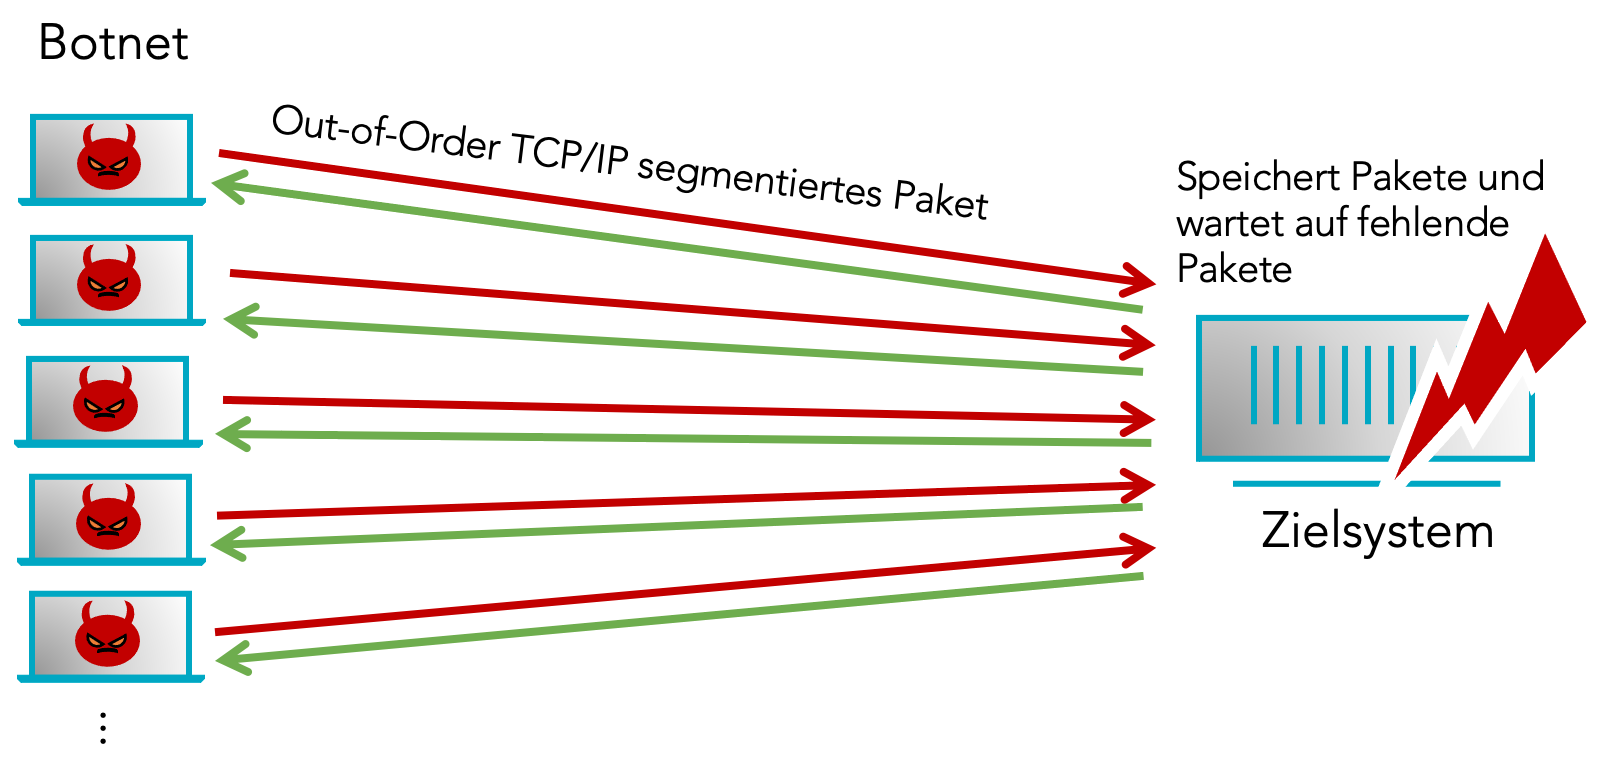
\includegraphics[width=0.9\linewidth]{img/seg}
	\end{center}
\end{frame}

\begin{frame}
	\frametitle{Abwehrmechanismen: Out-Of-Sequence-Attack}
	\begin{itemize}
		\item Puffern bis zu einer maximalen Anzahl an Segmenten pro Verbindung und insgesamt. Verwerfen von Segmenten sobald diese Anzahl erreicht ist.
	\end{itemize}
\end{frame}

\begin{frame}
	\frametitle{Ping of Death}
	\begin{center}
		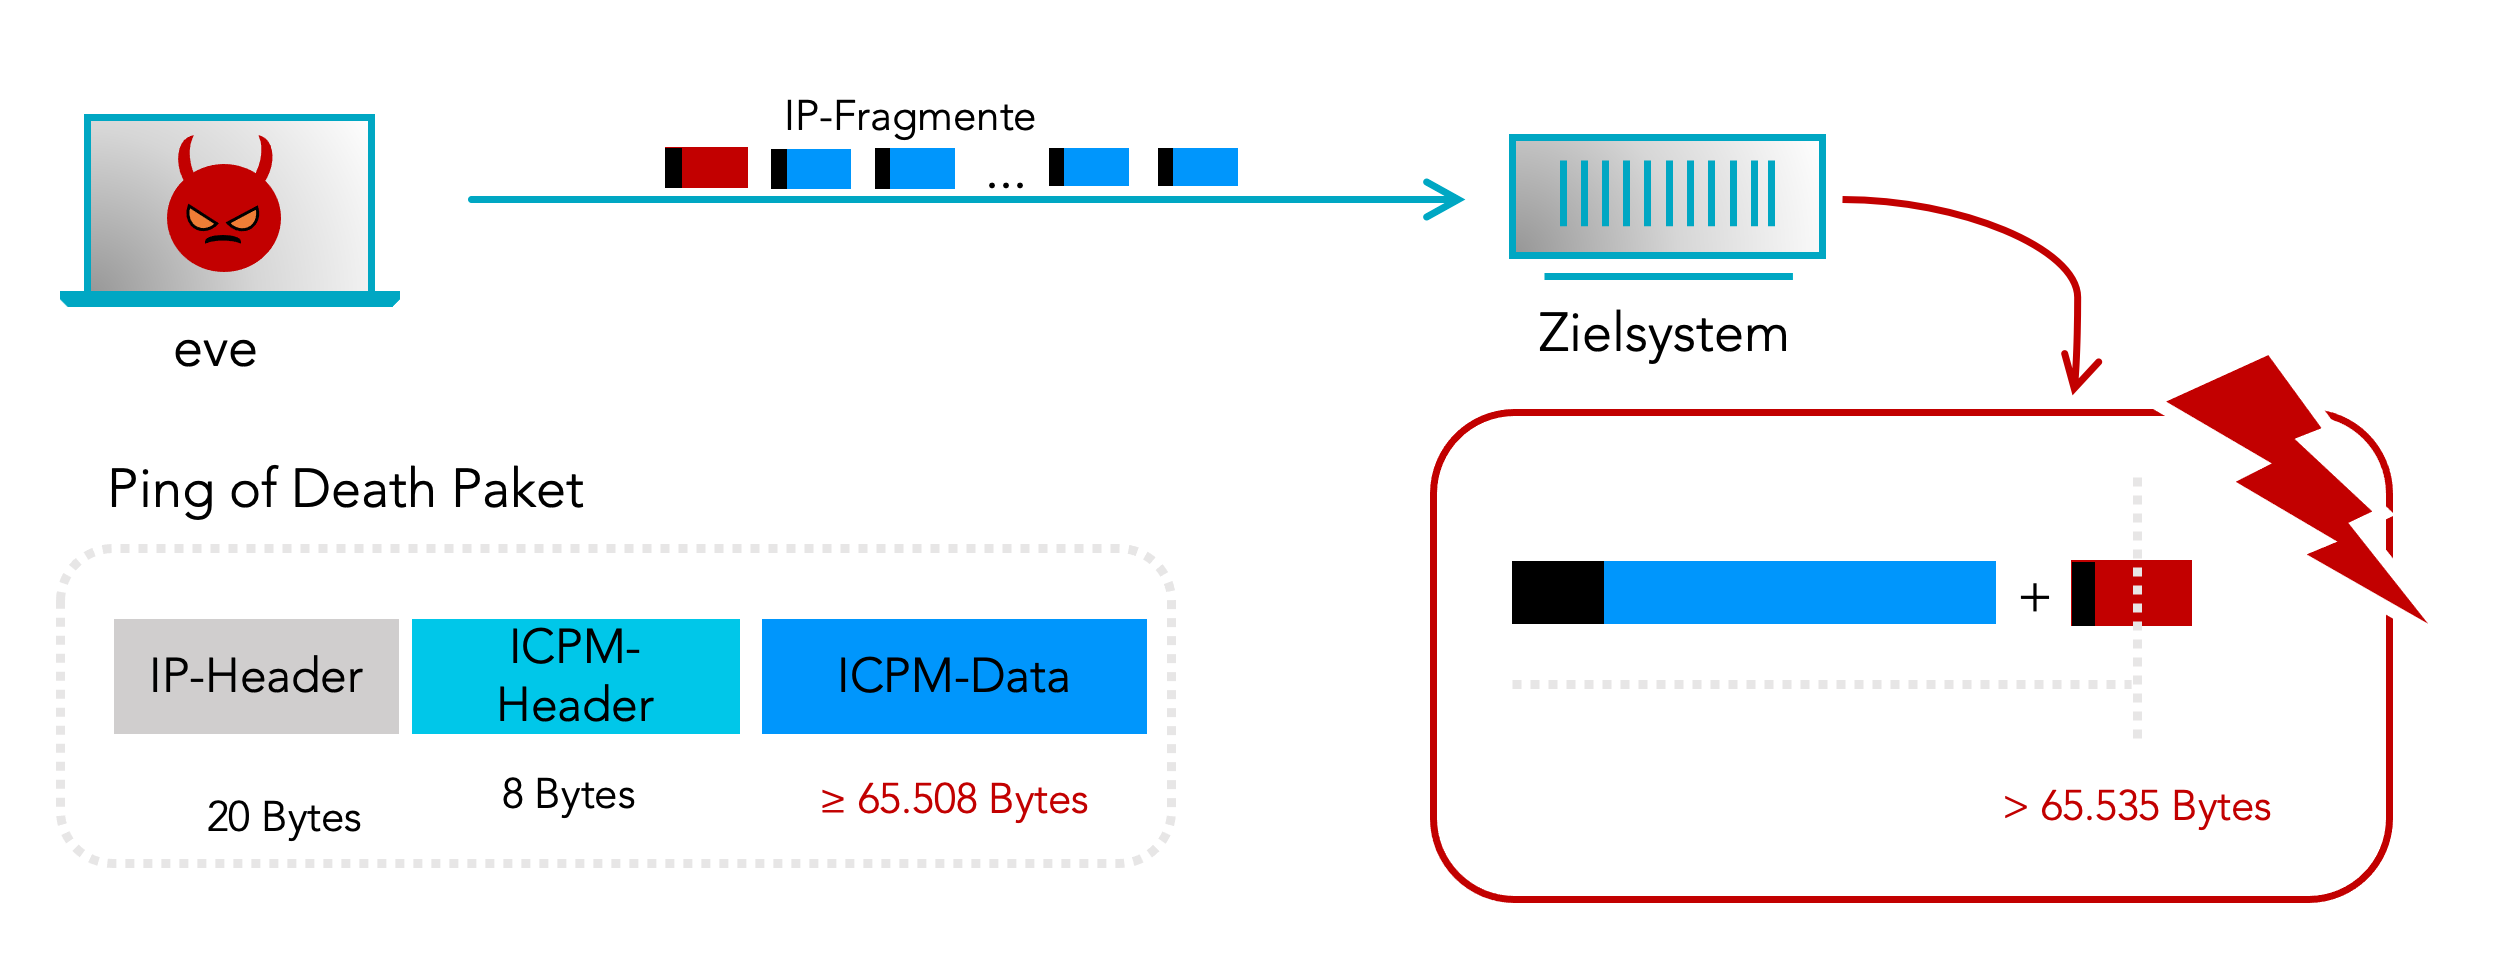
\includegraphics[width=0.9\linewidth]{img/5}
	\end{center}
\end{frame}

\begin{frame}
	\frametitle{Abwehrmechanismen: Ping of Death}
	\begin{itemize}
		\item Sicherstellung durch zusätzliche Checks, dass maximale Paketgröße beim Zusammenfügen der IP-Fragmente nicht überschritten wird
		\item Nutzung eines größeren Pufferspeichers
		\item Filterung bösartiger Pakete schon auf dem Weg durch das Netz: auf der Ebene von Routern und Firewalls oder durch Nutzung eines Content Delivery Networks \\ $\rightarrow$ Moderne Systeme i.d.R. gegen Ping of Death abgesichert \\ $\rightarrow$ Ping of Death stellt kaum noch eine Gefahr dar
	\end{itemize}
\end{frame}

\begin{frame}
	\frametitle{Ping Flood}
	\begin{center}
		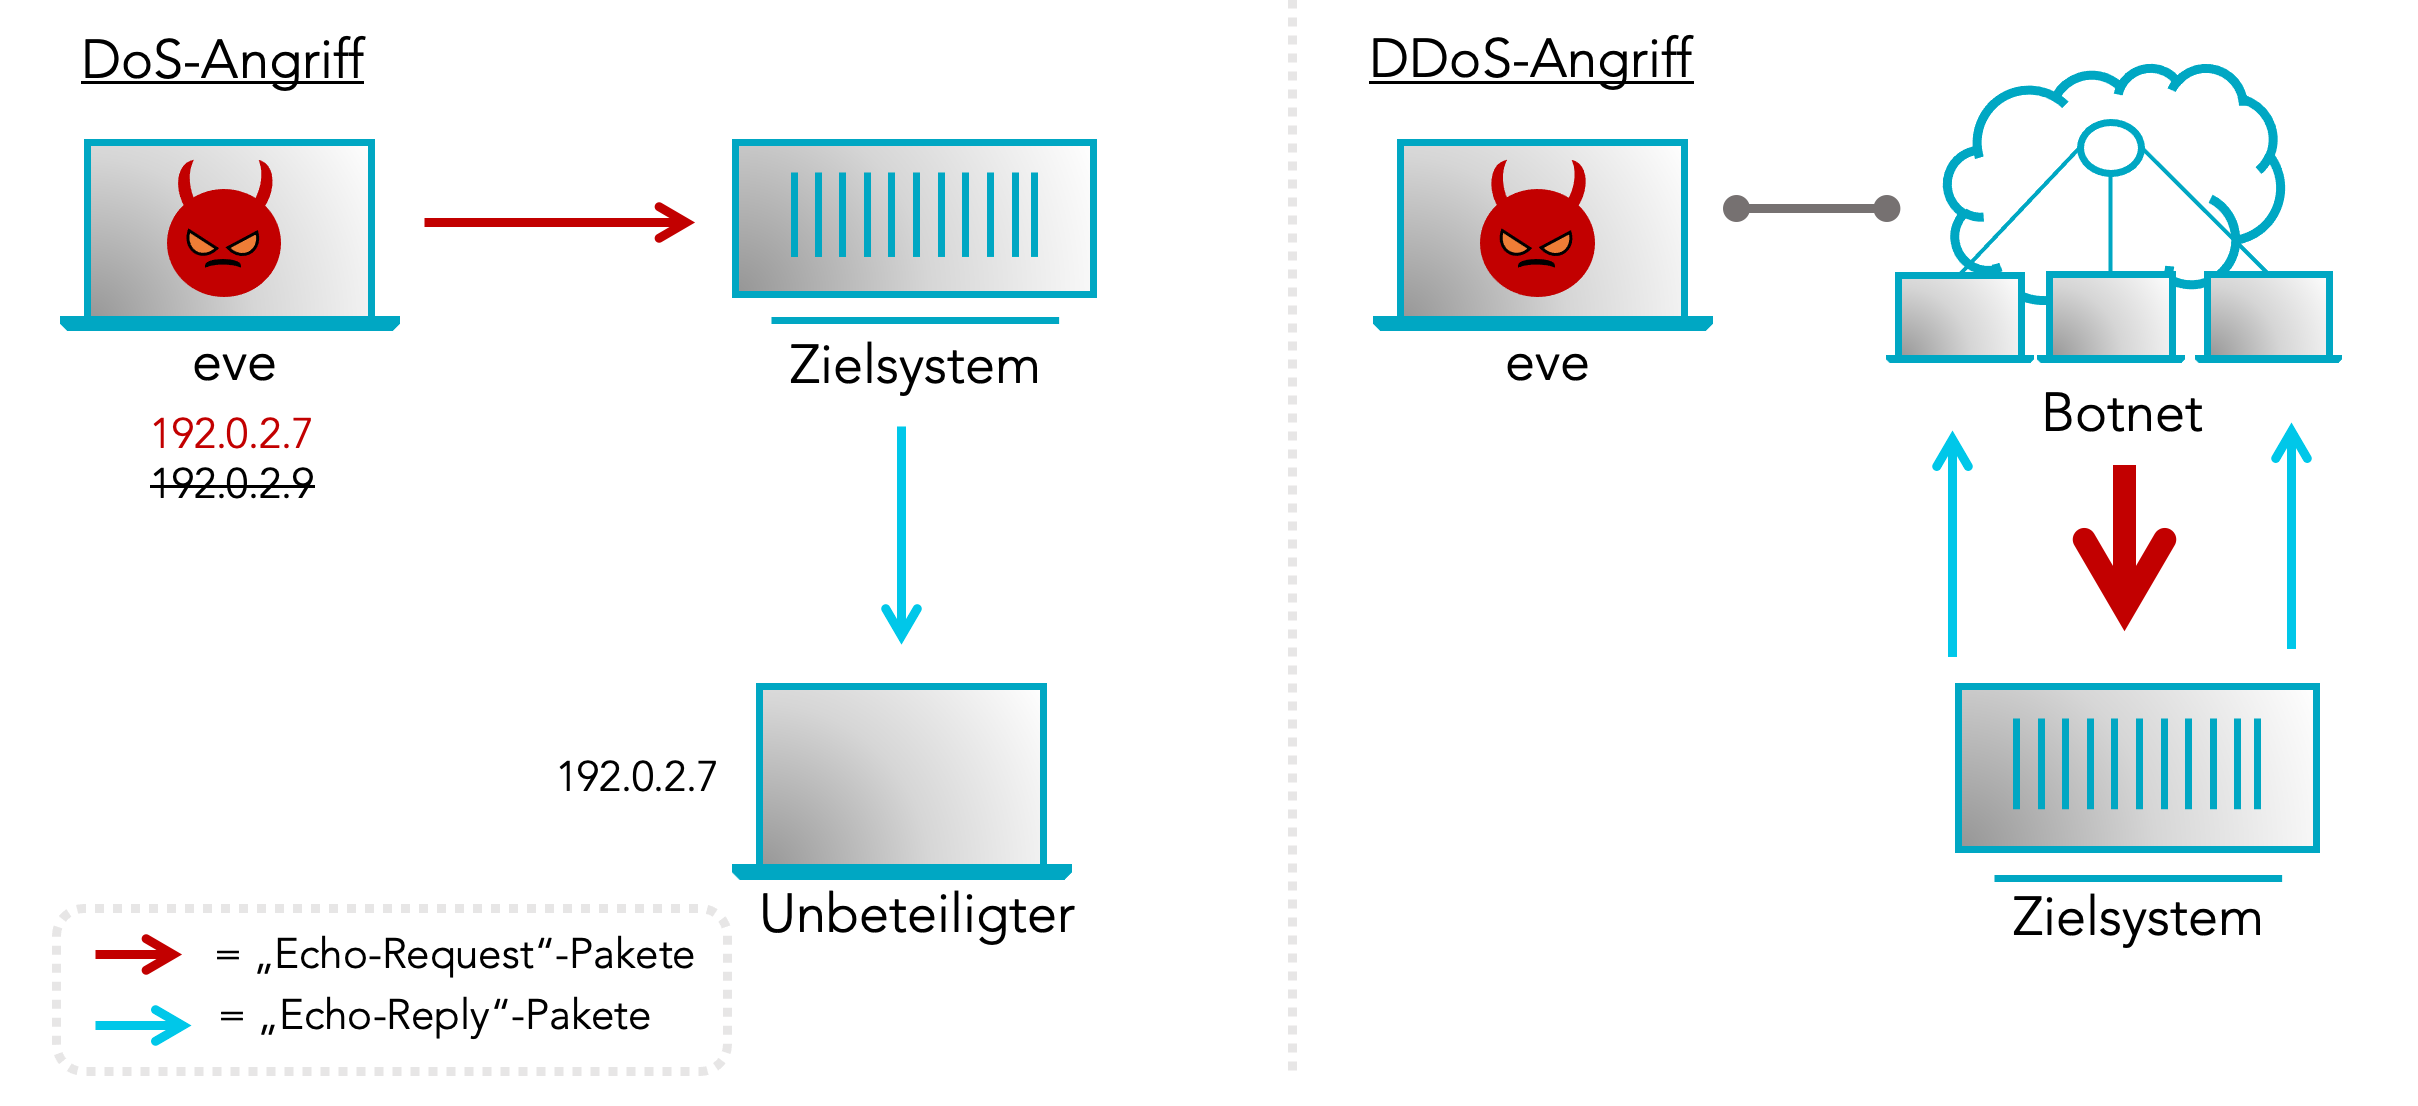
\includegraphics[width=0.9\linewidth]{img/6}
	\end{center}
\end{frame}

\begin{frame}
	\frametitle{Abwehrmechanismen: Ping Flood}
	\begin{itemize}
		\item Deaktivierung der ICMP-Funktionalität auf Opferseite
		\item Beschränkung der für ICMP-Nachrichten vorgehaltenen Bandbreite
	\end{itemize}
\end{frame}

\begin{frame}
	\frametitle{Smurf-Attack}
	\begin{center}
		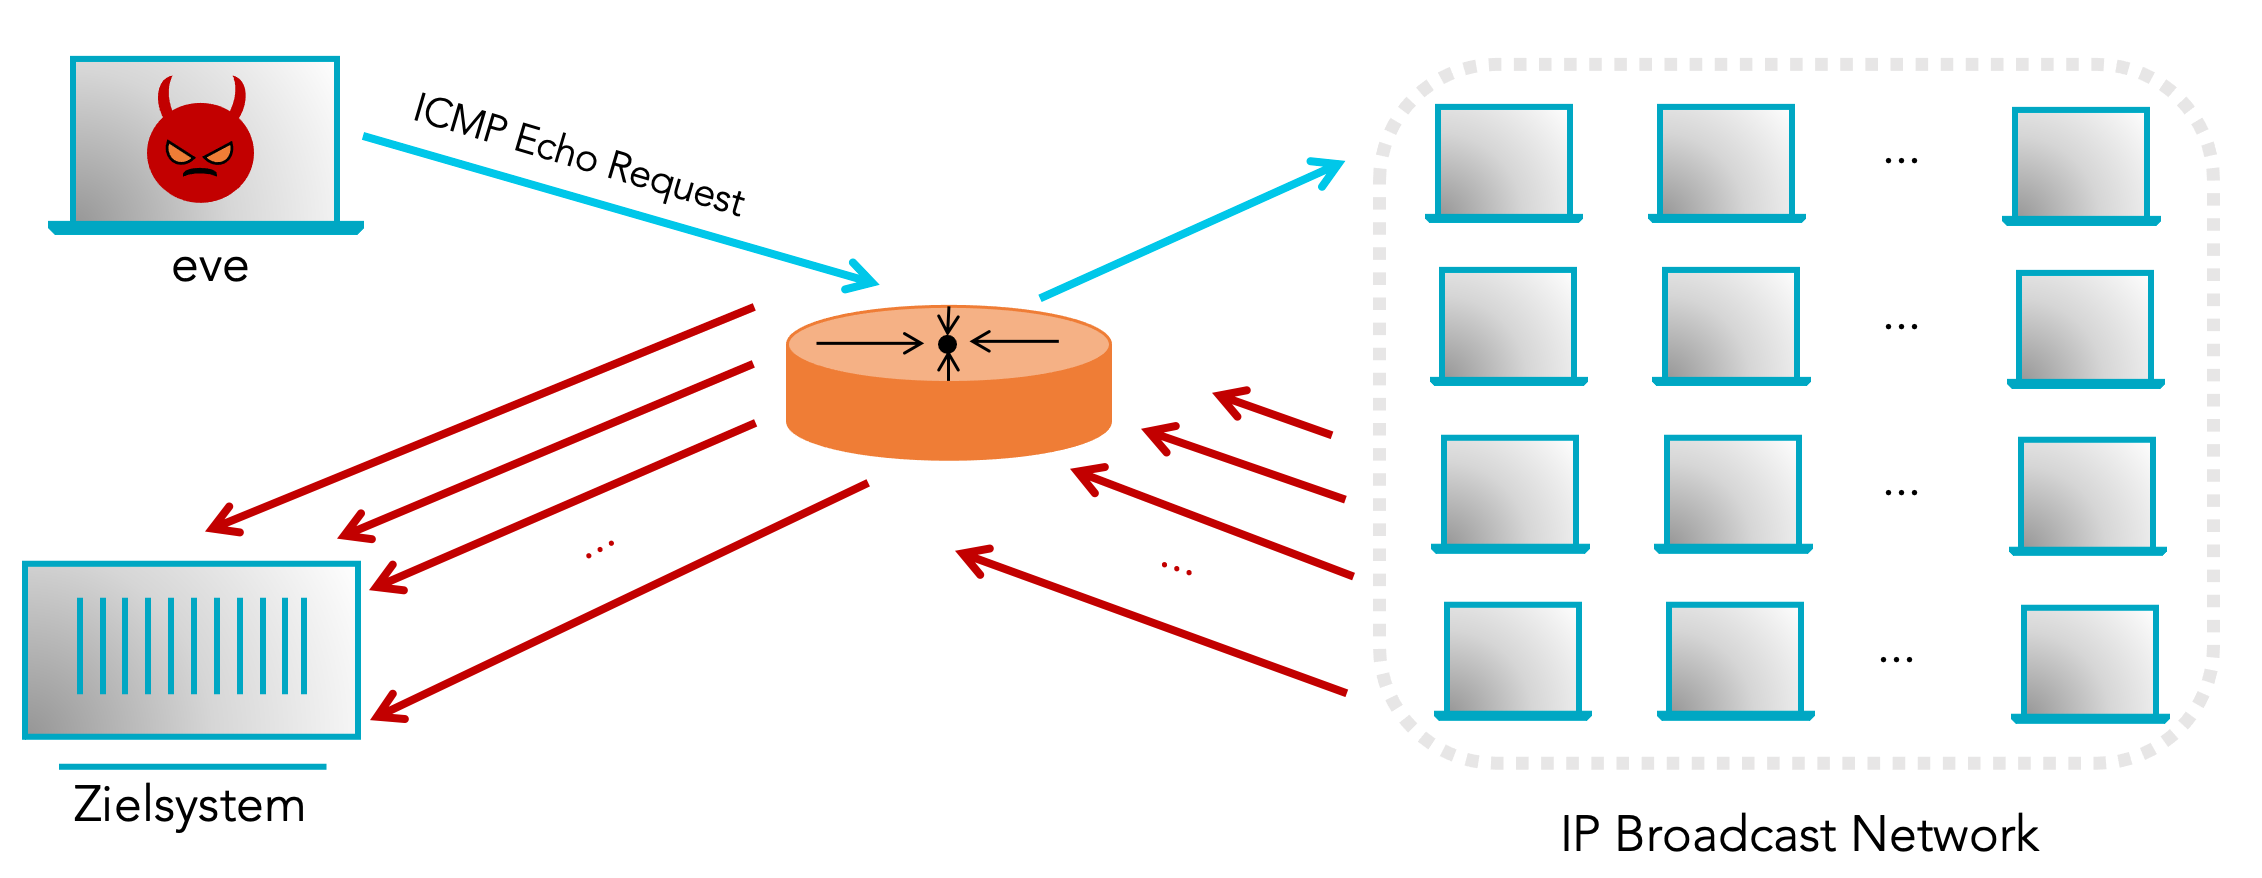
\includegraphics[width=0.9\linewidth]{img/smurf}
	\end{center}
\end{frame}

\begin{frame}
	\frametitle{Abwehrmechanismen: Smurf-Attack}
	\begin{itemize}
		\item Blockieren des im Netzwerk eingehenden gerichteten Broadcast-Verkehrs
		\item Konfiguration des Hosts und der Router so, dass sie nicht auf ICMP-Echo-Anfragen reagieren
	\end{itemize}
\end{frame}

\begin{frame}
	\frametitle{UDP-Flooding}
	\begin{center}
		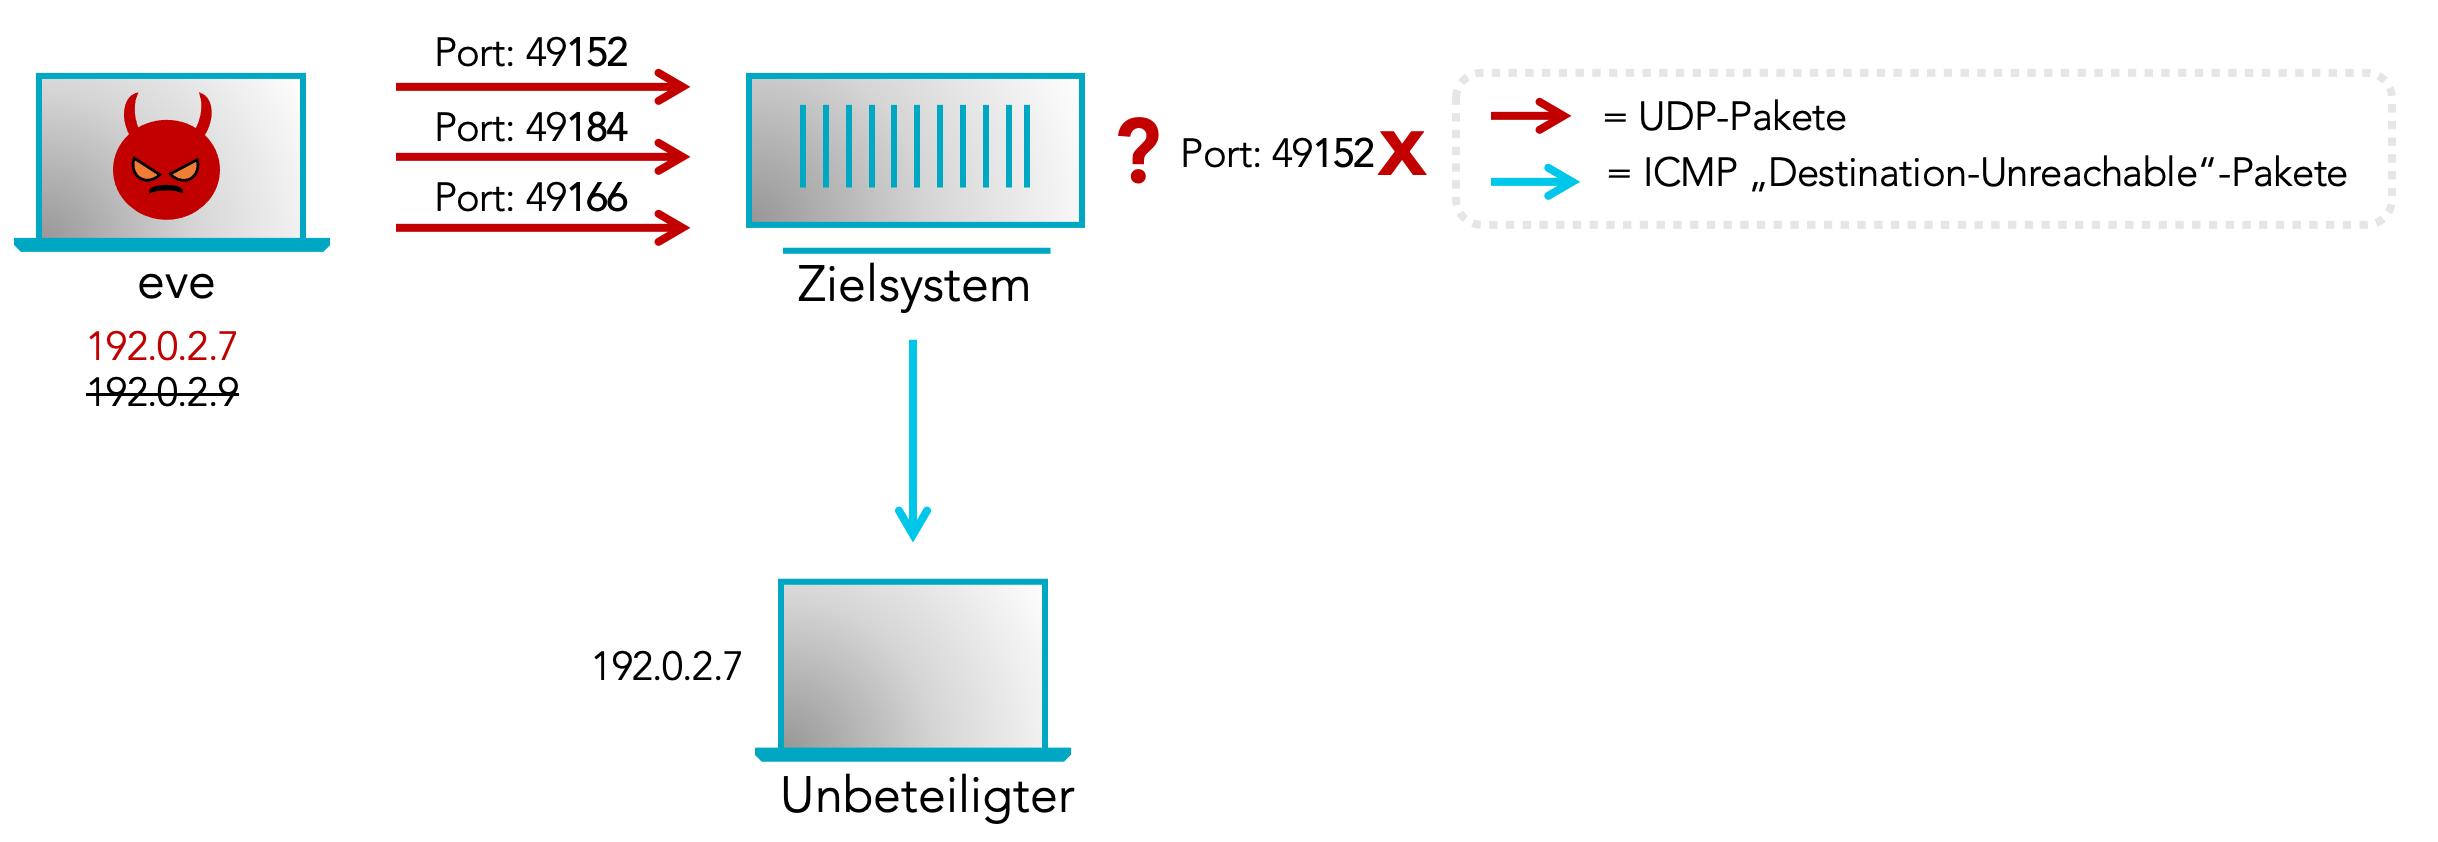
\includegraphics[width=0.9\linewidth]{img/udp}
	\end{center}
\end{frame}

\begin{frame}
	\frametitle{Abwehrmechanismen: UDP-Flooding}
	\begin{itemize}
		\item Durchsatzbegrenzung der ICMP-Antworten pro Zeiteinheit
		\item Filterung auf Firewall-Ebene auf dem Server
		\item Filtern von UDP-Paketen außer für DNS auf Netzwerk-Ebene
		\item Effizientere Datenstrukturen zur Verwaltung des Mappings von UDP Ports auf Anwendungen
	\end{itemize}
\end{frame}

\begin{frame}
	\frametitle{LAND Attack}
	\begin{center}
		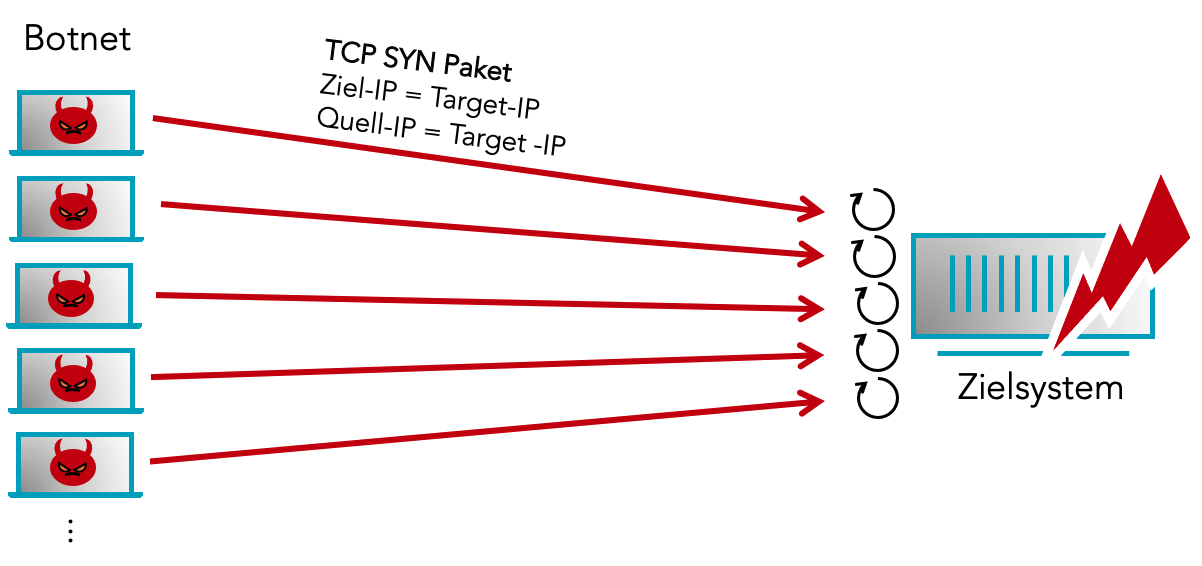
\includegraphics[width=0.9\linewidth]{img/Land}
	\end{center}
\end{frame}

\begin{frame}
	\frametitle{Abwehrmechanismen: LAND Attack}
	\begin{itemize}
		\item Verwerfen von Paketen, bei denen Absender und Empfänger gleich mir selbst sind
	\end{itemize}
\end{frame}

\begin{frame}
	\frametitle{Teardrop}
	\begin{center}
		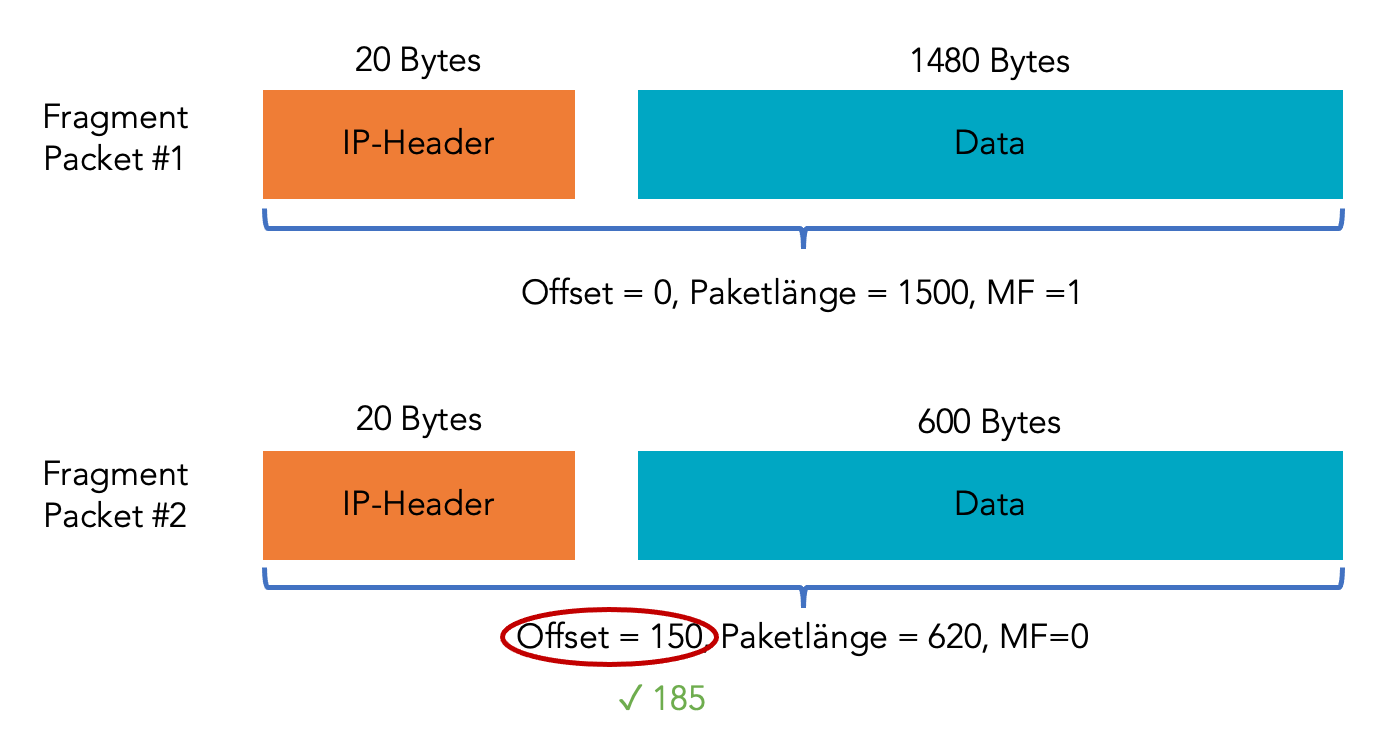
\includegraphics[width=0.9\linewidth]{img/TeardropAttack}
	\end{center}
\end{frame}

\begin{frame}
	\frametitle{Abwehrmechanismen: Teardrop}
	\begin{itemize}
		\item Inspektion ankommender Pakete auf Verletzung der Fragmentierungsregeln \\ $\rightarrow$ heute nicht mehr von Relevanz, wurde ca. 2000 gefixt
	\end{itemize}
\end{frame}

\begin{frame}
	\frametitle{Sockstress - TCP Zero Window}
	\begin{center}
		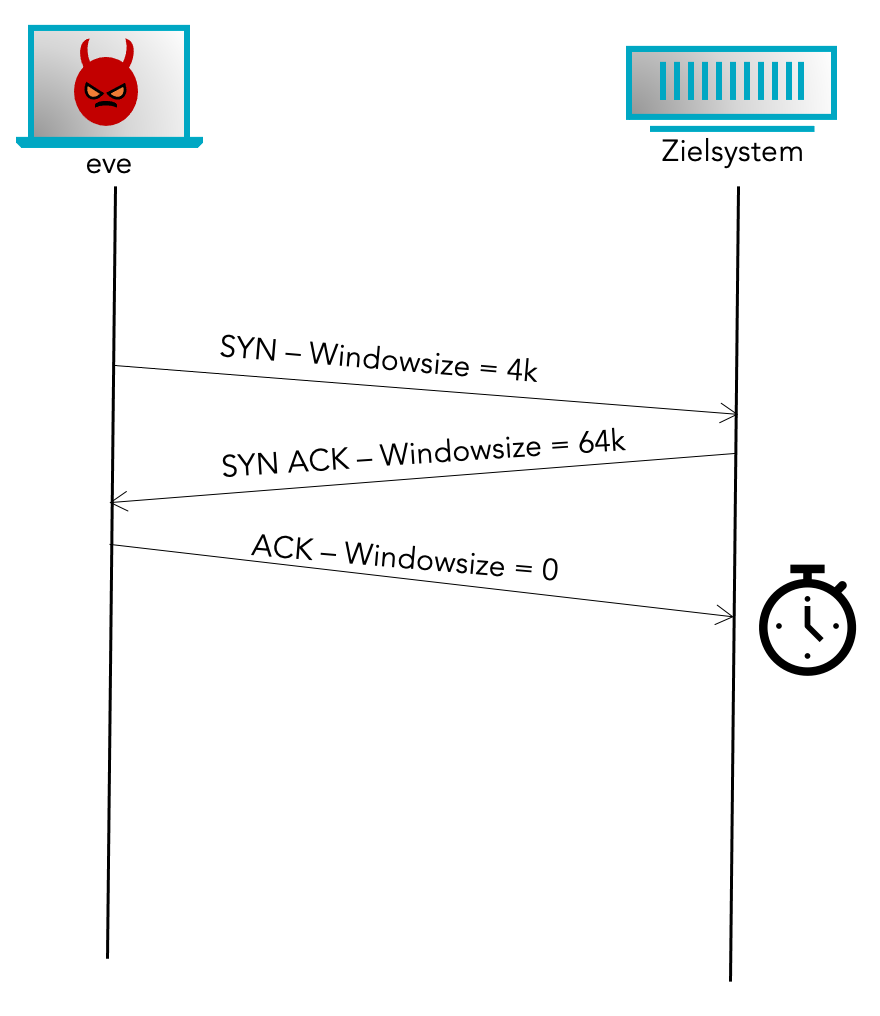
\includegraphics[width=0.6\linewidth]{img/zerowin}
	\end{center}
\end{frame}

\begin{frame}
	\frametitle{Sockstress - TCP Small Window}
	\begin{center}
		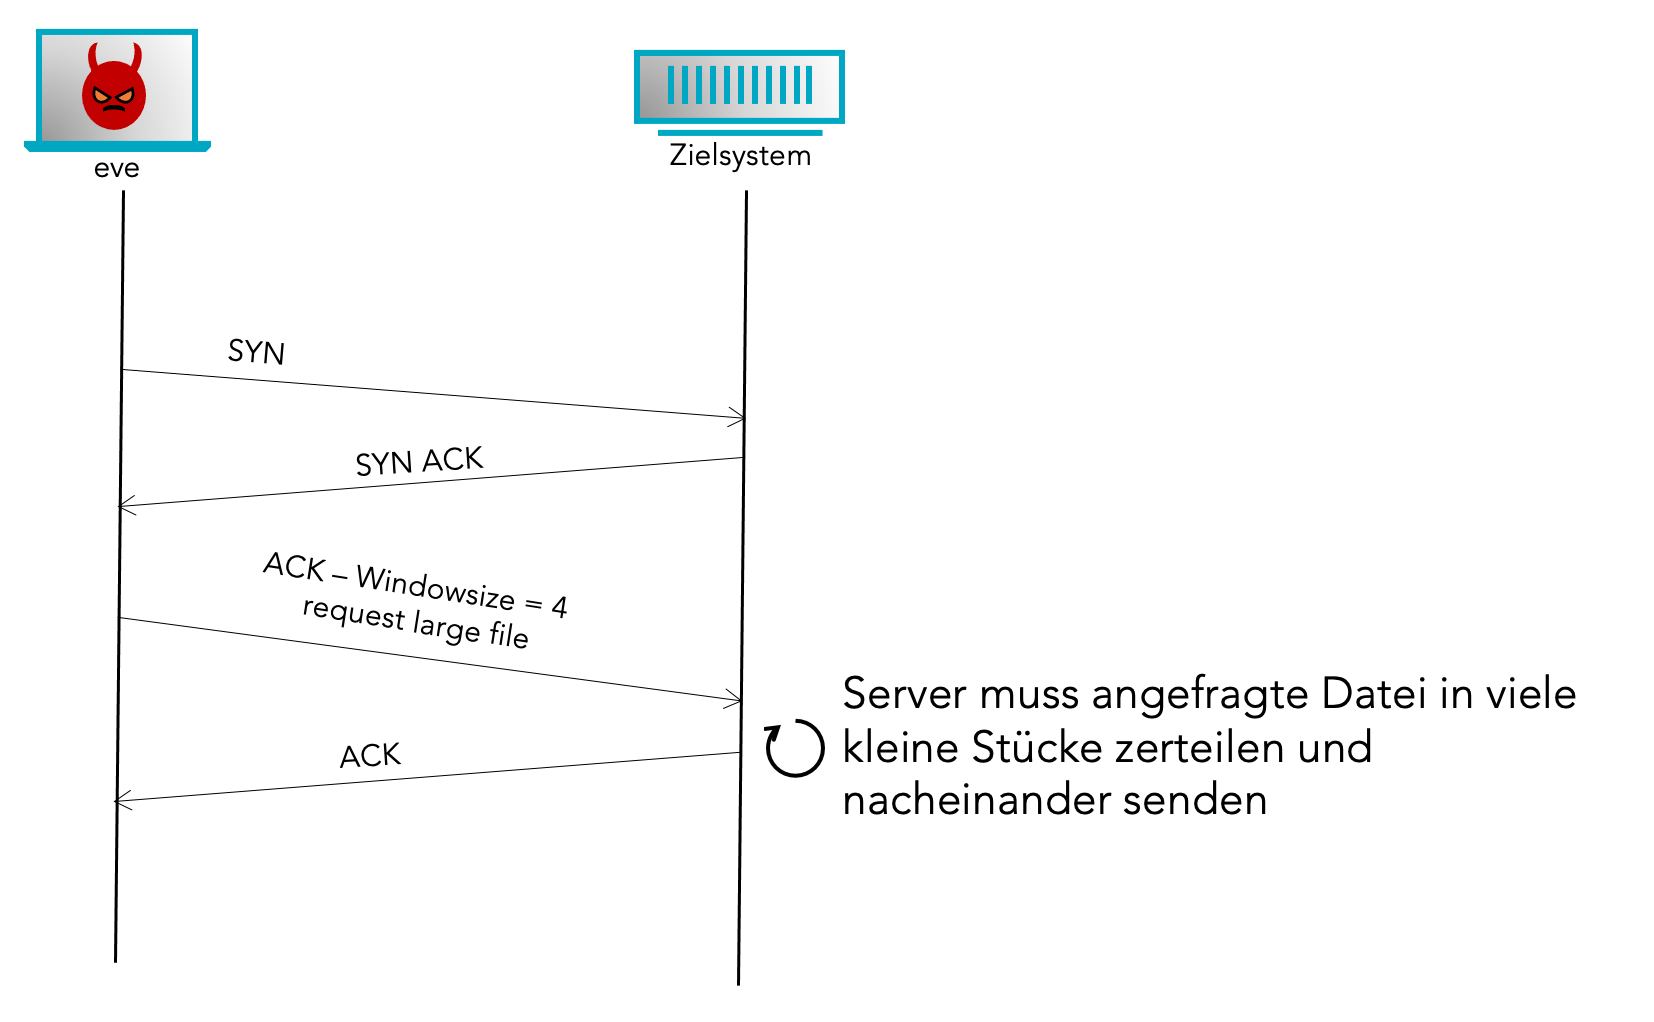
\includegraphics[width=1.0\linewidth]{img/smallwin}
	\end{center}
\end{frame}

\begin{frame}
	\frametitle{Abwehrmechanismen: Sockstress}
	\begin{itemize}
		\item Sockstress - Zero Window Connection Stress
		      \begin{itemize}
			      \item Verbot von TCP Verbindungen, welche bereits zu Beginn auf Windowsize = 0 setzen
			      \item Timer für Verbindungen mit Windowsize = 0 einführen
		      \end{itemize}
		\item Sockstress - Small Window Stress
		      \begin{itemize}
			      \item Effizientere Aufteilung großer Antworten bei kleinen Windows
		      \end{itemize}
	\end{itemize}
\end{frame}

\begin{frame}
	\frametitle{DNS Amplification Attack}
	\begin{center}
		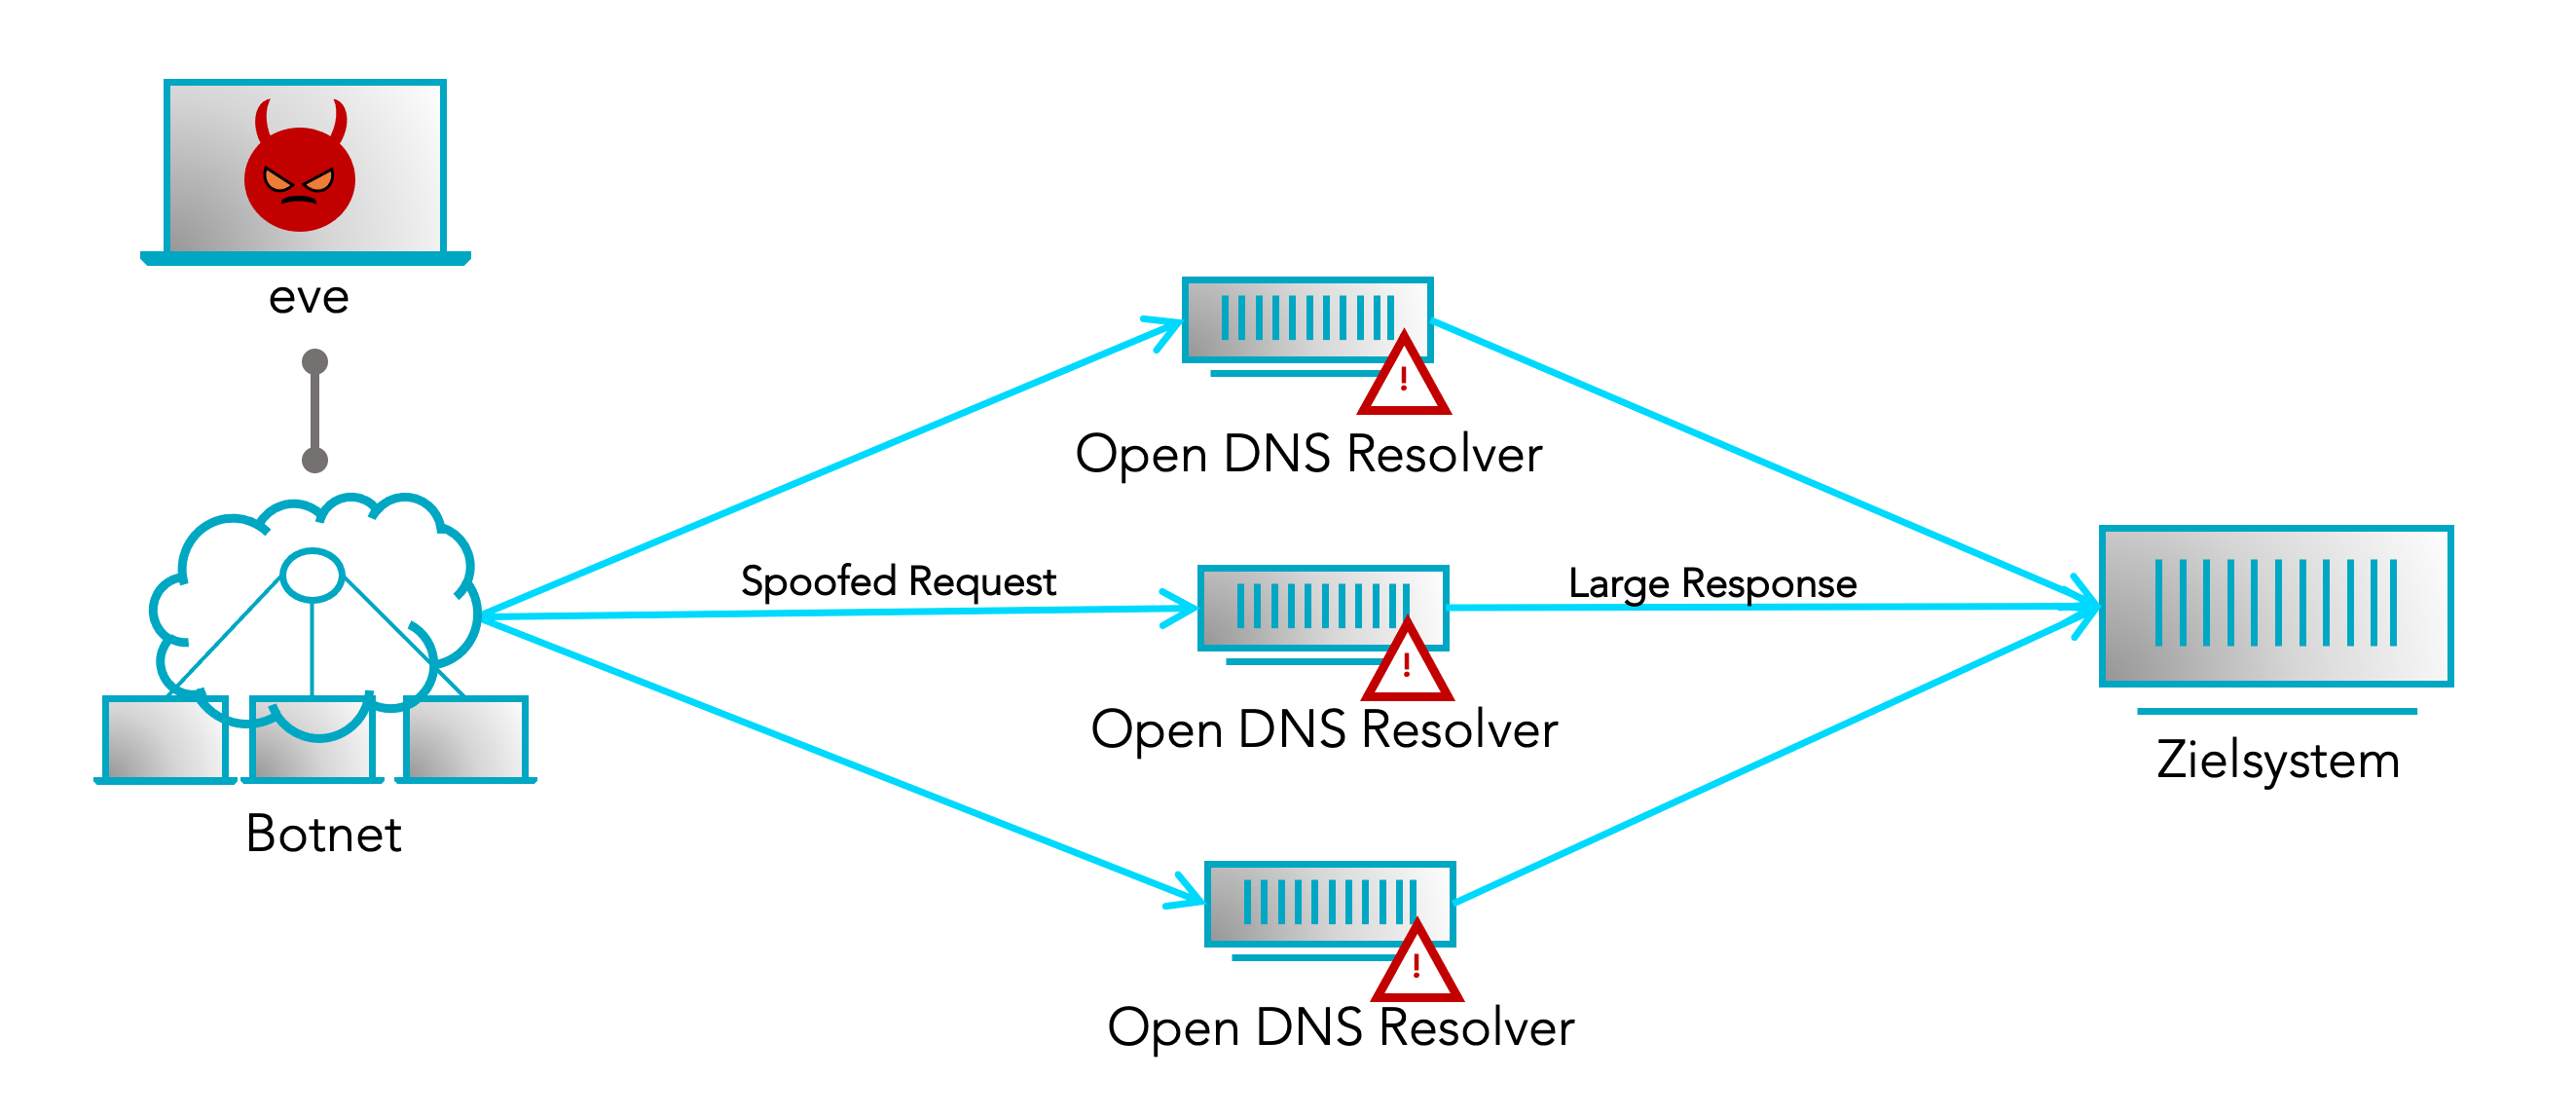
\includegraphics[width=1.0\linewidth]{img/DNSAmplificationAttack}
	\end{center}
\end{frame}

\begin{frame}
	\frametitle{Abwehrmechanismen: DNS Amplification Attack}
	\begin{itemize}
		\item Konfiguration lokaler DNS Server, sodass diese nur Anfragen von innerhalb der Organisation bearbeiten.
		\item Verwenden von DNS Anycast, um Anfragen zu verteilen und eine Überlast zu verhindern
	\end{itemize}
\end{frame}

\begin{frame}
	\frametitle{Auswirkungen}
	\begin{center}
		
\includegraphics[width=1.0\linewidth]{img/12}
	\end{center}
\end{frame}

\section{Erkennung von Attacken}
\begin{frame}
	\frametitle{Beispiel: SYN-Flooding}
	\begin{itemize}
		\item Extrem vereinfacht dargestellt
		\item[] sudo hping3 -c 15000 -d 120 -S -w 64 -p 80 --flood --rand-source 192.168.1.18
		      \begin{center}
			      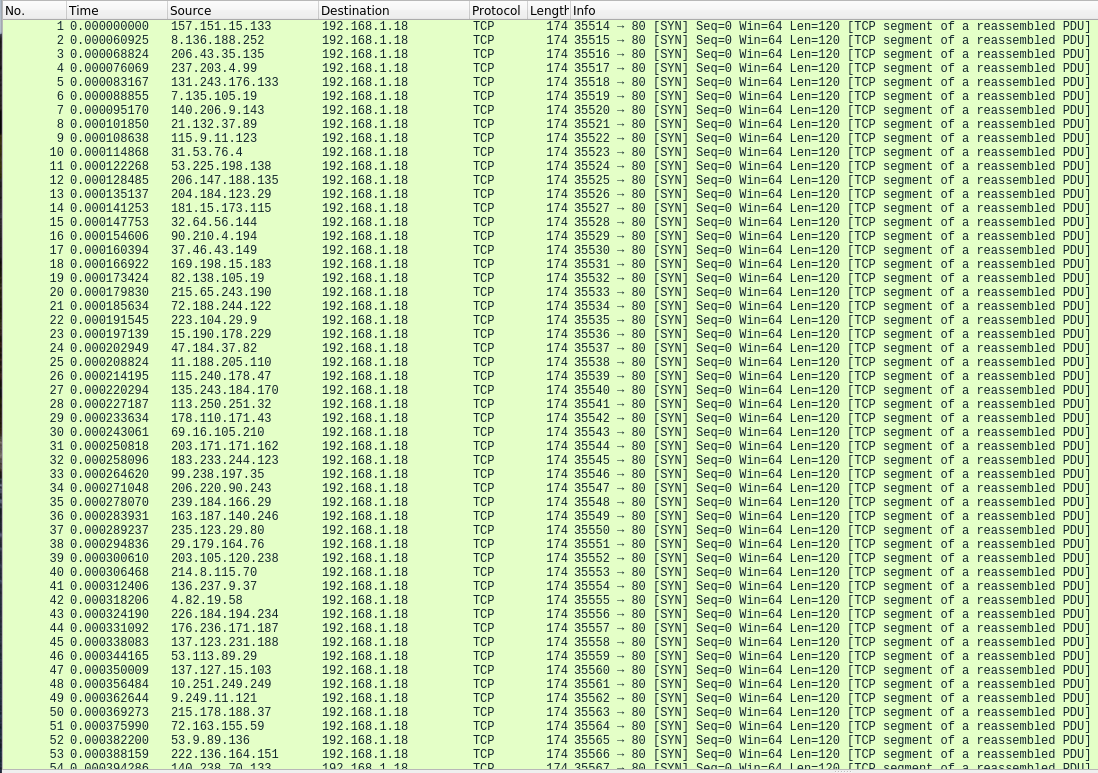
\includegraphics[width=0.7\linewidth]{img/14}
		      \end{center}
	\end{itemize}
\end{frame}

\section{Auswahl konkreter Angriffe}
\begin{frame}
	\frametitle{Relevante Angriffe}
	\begin{itemize}
		\item Angriffe höchster Priorität
		      \begin{itemize}
			      \item Alle Arten der SYN-Attacken
			      \item Sockstress
		      \end{itemize}
		\item Optionale Angriffsthemen
		      \begin{itemize}
			      \item UDP-Flooding
			      \item Out of Sequence Attack
			      \item LAND Attack
		      \end{itemize}
	\end{itemize}
\end{frame}

\end{document}